\Chapter{Physics of Liquid Scintillator Detectors}
\label{Ch5}

The PROSPECT AD reconstructs event energy by collecting light produced by the $^6$LiLS.
The PMTs of PROSPECT collect optical photons (photons with visible wavelength) from scintillation light yield. 
The light yield of the $^6$LiLS in response to an incident particle is not directly proportional to energy.
Instead, complicated molecular effects in the scintillator, called Birks' quenching, causes nonlinear energy response. 
Additional nonlinear light yield is contributed from the Cherenkov radiation of charged particles with high enough energy.
It is a vital step to understand the nonlinearity of light yield in PROSPECT to reconstruct particle energies and determine the absolute energy of $^{235}$U-produced \nuebar.

\Section{Organic Scintillator Light Yield}

The $^6$LiLS of PROSPECT AD is an organic scintillator.
The fluorescence process of organic scintillators is defined by the de-excitation photons of molecules from a variety of energy levels.
Particle energy is absorbed by a scintillator molecule to excite its electron configurations.
The de-excitation photon released by the excited molecule is the light yield of an organic scintillator.
The scintillation photon yield per incident energy, referred to as scintillation efficiency, is a vital property of a specific scintillator.
In an ideal energy-light conversion, the light yield with a scintillation efficiency $S$ can be expressed as
\begin{equation}
\frac{dL}{dx} = S(\frac{dE}{dx}).
\end{equation}
However, this efficiency is usually affected by radiationless de-excitation, such as molecular thermal motion, and light absorption by impurities, such as oxygen dissolved in an organic LS .
The mechanics of energy deposition in the scintillator differs with different types of particle interactions.

\Subsection{Beta Interactions}\label{sec:511}
Electron (betas) and positrons are the main subjects measured to reconstruct the reactor neutrinos' energy.
Only a small portion of the beta particle's kinetic energy is converted to the scintillation light. 
The major beta energy absorption mechanisms are the collision with atoms in the medium and the Bremsstrahlung effect.
Collisional loss is the major contributor for lower energy betas (below 10~MeV in $^6$LiLS), where the energy loss is due to ionization and excitation of the atoms in the medium.
The Bremsstrahlung effect absorbs electron/positron energy when the coulomb forces in the medium deflect it.
The energy loss of beta particles is commonly calculated based on the material compound components with the ESTAR database~\cite{bib:estar}, as shown in Figure~\ref{fig:EStar},
where the total energy loss is
\begin{equation}
\label{eq:dedx}
\frac{dE}{dx} = (\frac{dE}{dx})_c + (\frac{dE}{dx})_r.
\end{equation}
In the range of reactor neutrino produced IBD positron energy (0, 10) MeV, the major contributor of the positron energy loss is collisional loss. 
Because of the stopping power of the scintillator of PROSPECT, the length of the positron path is limited to a scale of several centimeters.

\begin{figure}[h!]
    \centering
    \includegraphics[width=0.7\textwidth]{Figures/ESTAR.png}\\
    \caption[Electron energy loss in $^6$LiLS]{The electron $dE/dx$ through $^6$LiLS calculated by E-star~\cite{bib:estar}.
    When electron energy is higher ($> 10$~MeV), the Brestrahlung effect contributes more significantly.}
    \label{fig:EStar}
\end{figure}

\Subsection{Muon Interactions}
Interactions absorbing the energy of cosmic muons is similar to beta particle interactions. 
Due to its high kinetic energy and mass-to-charge ratio, a cosmic muon can travel through multiple segments of the PROSPECT AD.
Occasionally, a Michel electron is generated when a muon decays inside of the detector volume.

\Subsection{Gamma Ray Interactions} 
Two gamma rays, each with 0.511~keV energy, are generated from the annihilation of an IBD positron.
The annihilation gamma events are part of the IBD prompt event along with positron kinetic energy deposition as described in Section~\ref{sec:511}.
Gamma energy is also utilized in energy scale calibration for PROSPECT.
Gamma interaction channels in scintillator include a photoelectric effect, Compton scattering, and electron-positron pair production.

Due to the photoelectric effect, gamma energy is partially absorbed by atoms in the medium.
Photo electrons (PEs) are emitted in the process when gamma energy overcomes the binding energy of the electron at its original shell. 
A PE's energy generally ranges from the scale of 1~keV to 10~keV.
The photoelectric effect is the major contributor causing energy loss of gamma rays with energy below 0.1~MeV.
If a single energy gamma loses all of its energy through photoelectric absorption, its energy deposition in a large detector volume would be a delta function.

The Compton scattering of a gamma photon also emits free electrons in the medium. 
The energies of the scattered electron and gamma are dependent on the scattering angle. 
Thus, the Compton recoil electron energy is a continuous spectrum for a single energy gamma-ray input.
The maximum energy of the Compton recoil electron is obtained when the scattering angle is maximized.
The energy difference between the incident gamma photon and the Compton recoil electron is given by
\begin{equation}
E_C \equiv E_\gamma  - E_{e^-} (\theta = \pi) = \frac{E_\gamma}{1+2E_\gamma/m_e}.
\end{equation}
The cross-section of Compton scattering as a function of the scattering angle is dependent on the medium's electron structure and density. 

When the energy of the incident gamma exceeds the 1.022~MeV energy threshold, the electron-positron pair production reaction can occur among the gamma ray interactions. 
Ideally, the total energy of the electron and positron pair equals the gamma energy.
The probability of pair production varies with respect to the absorber's atomic numbers.

The photoelectric effect mainly absorbs gamma energies below 0.1~MeV. 
When the energy of a gamma-ray exceeds the pair production threshold, pair production becomes a major cause for gamma energy loss in the higher energy range. 
The Compton scattering cross-section varies with gamma energy but becomes the most significant contributor of gamma energy absorption between 0.1~MeV to 10~MeV.
Hence, Compton scattering is the major cause of gamma energy loss in PROSPECT's IBD measurement.
Despite the type of interaction, a gamma photon energy is measured through its interaction generating electron and positrons.
Therefore, the PSD signature and the detector response to a gamma-ray is similar to a beta particle, with the exception that gamma-ray energy deposition spreads significantly farther in distance than an MeV-scale beta in organic scintillator.

\Subsection{Heavy Nucleon Interactions}
As described in Chapter~3, PROSPECT relies on the $n$-$^6$Li capture interaction to tag IBD event candidates. 
The alpha particle and triton products of the $n$-Li capture lose their energy as charged particles.

Charged heavy particle energy is absorbed through coulomb force interactions.
When charged nucleons enter media, the coulomb force between the nucleons and orbital electrons excites the electrons to higher energy states or ionizes the atom.
Thus, alpha particles, tritons, and protons excite scintillator molecules similar to electrons and positrons. 
For a 1~MeV scale charged nucleon, the energy loss $dE/dx$ is significantly higher because of the higher cross-section for ionization and collision with atoms.

Unlike particles described previously, neutrons do not deposit energy through ionization directly due to its neutral electrical charge.
Therefore, the neutron energy loss mechanism is dominated by interactions with charged particles.
In particular, fast neutrons can transfer kinetic energy to a proton, alpha particle or nucleus in the medium, causing a recoil of charged heavy particles.
During recoil interactions, fast neutrons are slowed down and eventually lose most of their kinetic energy.
The inelastic scattering between a neutron and another nucleus transfers neutron energy to the nucleus, which de-excites by emitting a gamma photon.
Thermal neutrons, with kinetic energy less than 0.025~eV, can be captured by proton-abundant atoms like hydrogen, boron, and lithium with high probability. 
Typical products of neutron capture are isotopes in excited states. 
De-excitation gamma photons from the product isotopes can be detected.
In the case of the $n$-Li capture process, an alpha particle and a Triton are generated.

\Section{Birks' Quenching}

A scintillator's light yield is ideally proportional to the energy loss as in Eq.~\ref{eq:dedx}.
In reality, the quenching effect in an organic scintillator causes nonlinear light yield with respect to the energy deposition.
Multiple factors affect the quenching effect, including radiationless molecular movements and the impurities in components absorbing the energy of scintillation light.
A semi-empirical light yield conversion was developed by Birks~\cite{bib:birks, bib:birksbook}. 
This conversion is referred to as Birks' Law, which is based on experimental measurement of organic scintillators' light yields and the theoretical assumption that the quenching effect varies with incident event ionization density. 
Birks' Law of scintillator quenching is expressed as
\begin{equation}
\frac{dL}{dx} = \frac{S\frac{dE}{dx}}{1+k_{B1}\frac{dE}{dx} + k_{B2}(\frac{dE}{dx})^2},
\end{equation}
where $k_{B1}$ and $k_{B2}$ are the first and second order Birks' constants that vary for different scintillators.
Nonlinearity of light yield is severe at lower energies near the Bragg peak of the concerned particle. 

Birks' Law also indicates significantly lower light yield from incident particles with high $\frac{dE}{dx}$.
Thus, the effective light yield efficiency from protons and alpha particles is generally lower than electrons and gamma photons, resulting in severe differences between experiment-reconstructed energy and the actual deposited energy.
The reconstructed energy is hence referred to as MeV electron equivalent (MeVee).
For instance, the total energy of the alpha particle and Triton from $n$-Li capture is 4.78~MeV, while its PROSPECT detector reconstructed energy is $\sim$0.55~MeVee.
The nonlinear scintillation response to different particles with various energy is shown in Figure~\ref{fig:birks}.

\begin{figure}[h!]
    \centering
    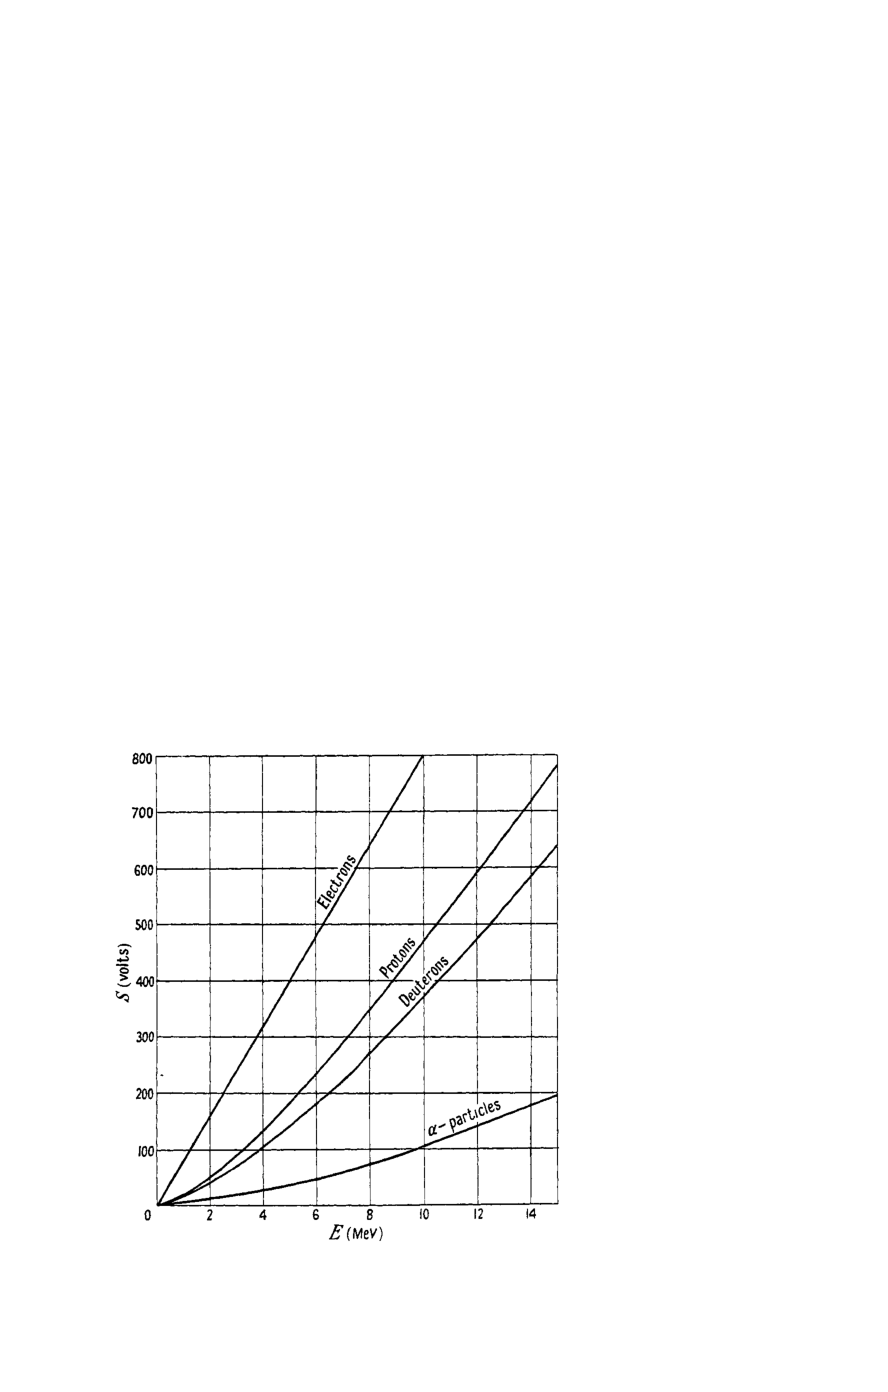
\includegraphics[width=0.55\textwidth]{Figures/BirksNonlinearHigh.pdf}
    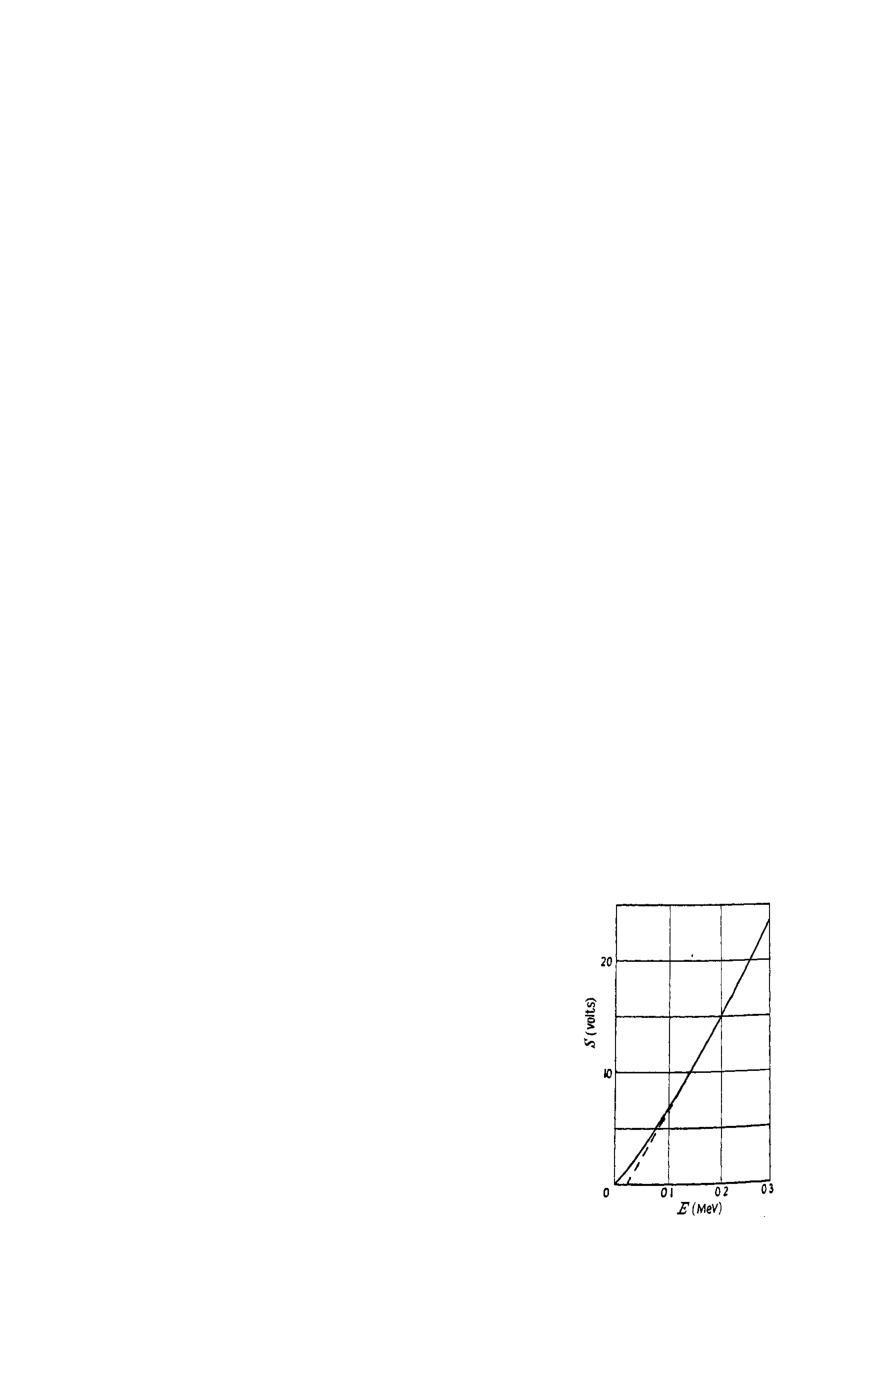
\includegraphics[width=0.38\textwidth]{Figures/BirksNonlinearLow.pdf}
    \caption[Quenched scintillator light response]{
     (Left)The nonlinear scintillator response to different particle types~\cite{bib:birks}.
	(Right) The light response of a scintillator to low energy electrons.
    $S$ is the light signal output of Birks' measurement with organic scintillator anthracene.
    Because of high $dE/dx$, protons and alpha particles produce significantly less scintilation light per MeV, compared to an electron.
    }
    \label{fig:birks}
\end{figure}

Different scintillators have unique sets the Birks' quenching constants $k_{B1}$ and $k_{B2}$.
Measurements of $k_{B1}$ and $k_{B2}$ are usually made by comparing the electron and heavy-ion light yields at constant incident energy.
However, the measured quenching constants are particularly challenging to simulate in most experiments due to large uncertainty of $dE/dx$ calculation in MC simulations.
The method used in PROSPECT simulations is discussed in Chapters~\ref{Ch6} and \ref{Ch7}.

\Section{Cherenkov Radiation}
Photons produced through Cherenkov radiation~\cite{bib:ckov} are another source of light in PROSPECT.
When a charged particle's speed in a medium is higher than the phase speed of light, a Cherenkov photon is emitted as the polarizable medium molecules are polarized by the charged particle.
Coherent light is radiated at an angle with respect to the particle's traveling direction and speed.
The number of photons generated in Cherenkov radiation is 
\begin{equation}
    \frac{d^2N}{dxd\lambda} = \frac{2\pi\alpha z^2}{\lambda}\left(1- \frac{1}{\beta^2n^2(\lambda)}\right),
\end{equation}
where $N$ is number of photons, $\alpha$ is the fine structure constant, $z$ is the particle's electric charge, $\beta$ is the speed of the particle, and $n(\lambda)$ is the index of refraction of the medium.
The actual optical spectrum of the Cherenkov light is dependent on the scintillator index of refraction, transmission efficiency, and absorbance.
The thresholds of Cherenkov radiation production for electrons and gammas are shown in Figure~\ref{fig:ckovthresh}, where the threshold for electrons is $\sim$0.2~MeV when the medium index of refraction is 1.5.

\begin{figure}[h!]
    \centering
    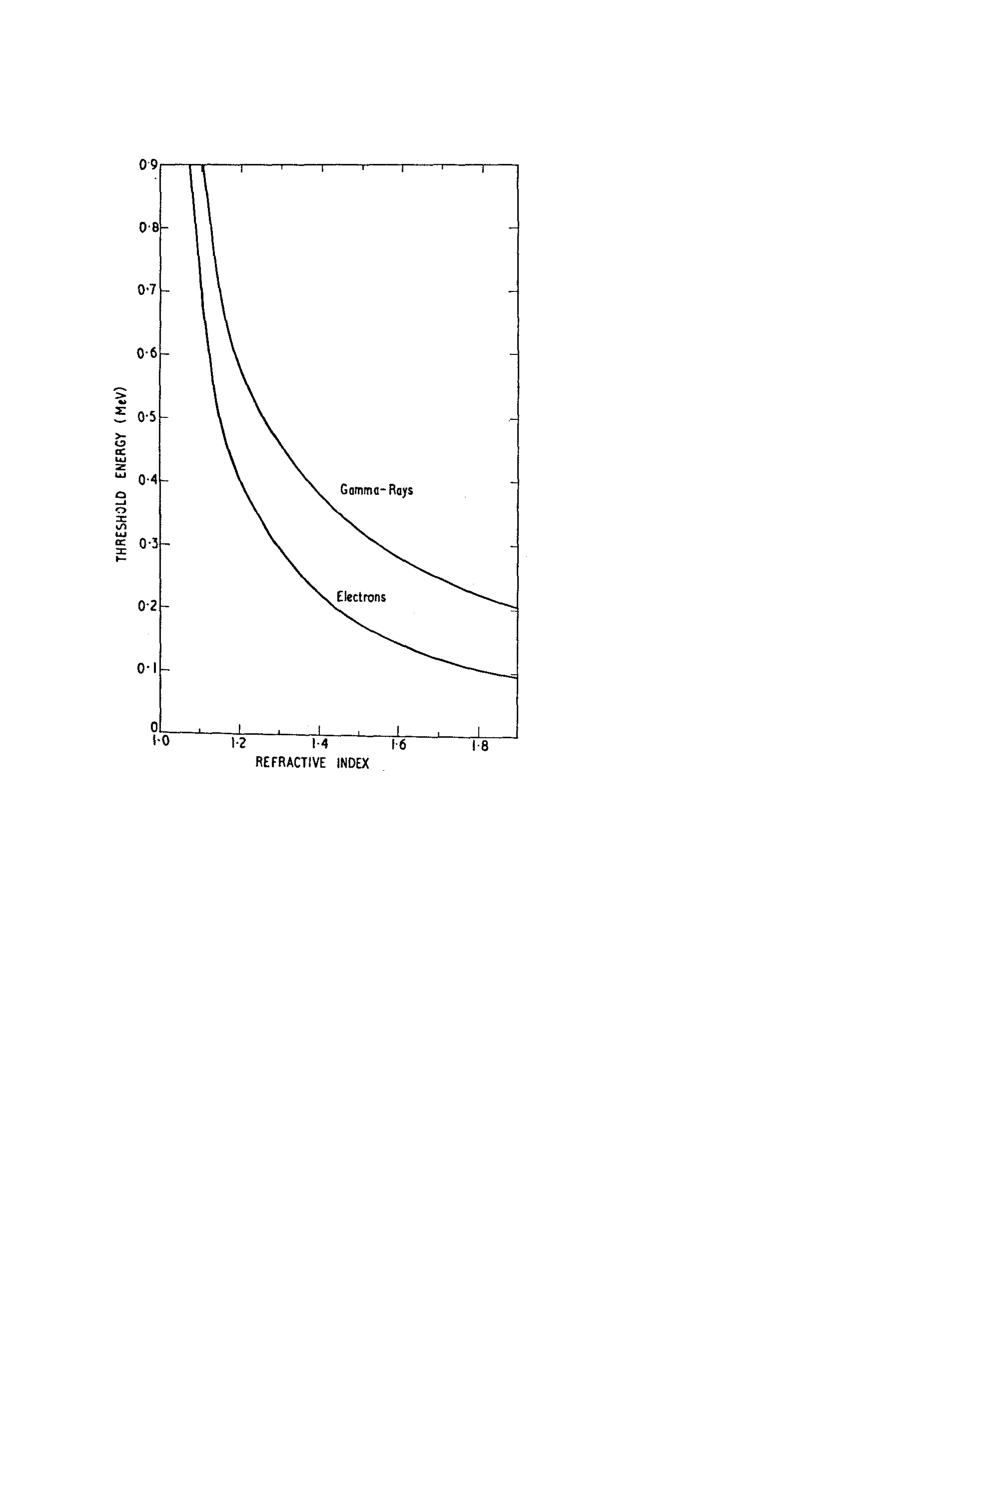
\includegraphics[width=0.5\textwidth]{Figures/CkovThresh.pdf}
	\caption[Cherenkov radiation thresholds]{
    The Cherenkov radiation thresholds of gammas and electrons in media with different indices of refraction.}
    \label{fig:ckovthresh}
\end{figure}

Cherenkov radiation of charged particles produce prompt photons in the PROSPECT AD that is indistinguishable from scintillation light.
The nonlinear energy response caused by Cherenkov radiation is discussed in Chapters~\ref{Ch6} and \ref{Ch7}.
